%% Overleaf			
%% Software Manual og Technical Document Template	
%% 									
%% This provides an example of a software manual created in Overleaf.

\documentclass{ol-softwaremanual}

% Packages used in this example
\usepackage{graphicx}  % for including images
\usepackage{microtype} % for typographical enhancements
\usepackage{listings}    % for code listings
\usepackage{amsmath}   % for equations og mathematics

\usepackage[a4paper,top=4.2cm,bottom=4.2cm,left=3.5cm,right=3.5cm]{geometry} % forsatt ting page size og margins
\usepackage{xcolor}
\usepackage{appendix}
\usepackage[norsk]{babel}
\usepackage[T1]{fontenc}
\usepackage{float}
\usepackage{enumitem}
\usepackage{multicol}
\usepackage[inkscapelatex=false]{svg}
\usepackage{pdfpages,caption,geometry}
\usepackage{hyperref}
\usepackage[acronyms]{glossaries}
\usepackage{bookmark}
% Custom macros used in this example document
\newcommand{\doclink}[2]{\href{#1}{#2}\footnote{\url{#1}}}
\newcommand{\cs}[1]{\texttt{\textbackslash #1}}
\definecolor{codegreen}{rgb}{0,0.6,0}
\definecolor{codegray}{rgb}{0.5,0.5,0.5}
\definecolor{codepurple}{rgb}{0.502,0.502,0.0}
\definecolor{backcolour}{rgb}{0.95,0.95,0.95}
\renewcommand*{\lstlistlistingname}{Code snippets}
\newcommand{\figref}[1]{Figur~\ref{#1}}
\newcommand{\true}{\textbf{TRUE} }
\newcommand{\false}{\textbf{FALSE} }
\glsaddkey*
{et}% key
{\glsentrytext{\glslabel}et}% default value
{\glsentryet}% command analogous til \glsentrytext
{\Glsentryet}% command analogous til \Glsentrytext
{\glset}% command analogous til \glstext
{\Glset}% command analogous til \Glstext
{\GLSet}% command analogous til \GLStext
\glsaddkey*
{sk}% key
{\glsentrytext{\glslabel}sk}% default value
{\glsentrysk}% command analogous til \glsentrytext
{\Glsentrysk}% command analogous til \Glsentrytext
{\glssk}% command analogous til \glstext
{\Glssk}% command analogous til \Glstext
{\GLSsk}% command analogous til \GLStext
\glsaddkey*
{ske}% key
{\glsentrytext{\glslabel}ske}% default value
{\glsentryske}% command analogous til \glsentrytext
{\Glsentryske}% command analogous til \Glsentrytext
{\glsske}% command analogous til \glstext
{\Glsske}% command analogous til \Glstext
{\GLSske}% command analogous til \GLStext

\glsaddkey*
{en}% key
{\glsentrytext{\glslabel}en}% default value
{\glsentryen}% command analogous til \glsentrytext
{\Glsentryen}% command analogous til \Glsentrytext
{\glsen}% command analogous til \glstext
{\Glsen}% command analogous til \Glstext
{\GLSen}% command analogous til \GLStext
\lstdefinelanguage{ST}
{
	morekeywords={
	case,of,if,then,end_if,end_case,super,function_block,extends,var,
	constant, byte,,end_var,var_input, real,bool,var_output,
	dint,udint,word,dword,array, of,uint,not,adr, program, for, end_for, while, do, end_while, repeat, end_repeat, until, to, by, else, elsif, var_in_out,or
	},
	otherkeywords={
		:, :=, <>,;,\,.,\[,\],\^,1,2,3,4,5,6,7,8,9,0,TRUE, FALSE, \{attribute,  \'hide\'\}
	},
	keywords=[1]{
		case,of,if,or,then,end_if,end_case,super,function_block,extends,var,
		constant, byte,,end_var,var_input, real,bool,var_output,
		dint,udint,word,dword,array, of,uint,not,adr, :, :=, <>,;,\,.,\[,\],\^,program, for, end_for, while, do, end_while, repeat, end_repeat, until, to, by, else, elsif, var_in_out
	},
	keywordstyle=[1]\color{blue},
	keywords=[2]{
		1,2,3,4,5,6,7,8,9,0, TRUE, FALSE
	},
	keywordstyle=[2]\color{codepurple},
	keywords=[3]{
		\{attribute,  \'hide\'\}
	},
	keywordstyle=[3]\color{codegray},
	sensitive=false,
	morecomment=[l]{//}, 
	morecomment=[s]{(*}{*)},
	morestring=[b]{"},
	morestring=[b]{'}
}

\lstset{
	language={ST},
	backgroundcolor=\color{backcolour},
	commentstyle=\color{codegreen}\textit,
	keywordstyle=\color{blue},
	numberstyle=\tiny\color{codegray},
	stringstyle=\color{codepurple},
	basicstyle=\ttfamily\scriptsize,
	breakatwhitespace=false,         
	breaklines=true,                 
	captionpos=b,                    
	keepspaces=true,                 
	numbers=left,                    
	numbersep=5pt,                  
	showspaces=false,                
	showstringspaces=false,
	showtabs=false,                  
	tabsize=2
}
% Frontmatter data; appears on title page
\title{Torsjonsrigg\\Dokumentasjon}
\version{1.1.2}
\author{Vebjørn Steinsholt}
\softwarelogo{
\includegraphics[width=8cm]{Pictures/logo.png}}
\makeglossaries
\begin{document}

\maketitle

\tableofcontents
\listoffigures
\lstlistoflistings
\newpage

\section{Introduksjon}

Dette dokumentet er ment som en grundig dokumentasjon av både maskinvare, mekaniske deler og programvare som tilhører torsjonsriggen. Den inneholder detaljerte beskrivelser, instrukser for bruk og tekniske spesifikasjoner slik at man kan gjennomføre korrekt oppsett, bruk, vedlikehold og de rette sikkerhetstiltakene. Om du er student, forsker, ingeniør eller tekniker, skal dette dokumentet støtte opp om ditt arbeid ved å gi deg klar og konsis informasjon om riggens kapasiteter og funksjonalitet.
\section{Mekanisk}
\footnote{Designet av Emil Bratlie} \footnote{bygget av Gisle Martin Pettersen Haugseth}
\subsection{Sikkerhet}
Før alt arbeid og rigging skal man sørge for at styringen/elektriske delen/annet bedre navn? til riggen er avslått og gjort strømløs, slik at man fjerner risikoen for at maskineriet begynner å snurre mens man er i nærheten/jobber på det, samtidig som man fjerner risikoen for strømgjennomføring.

Disse punktene er viktige da vi hverken har kontroll på om skapet må godkjennes eller ikke enda, og vi ikke har fått sikret at det er nok med å koble inn nødstopp før rigging enda.

Alt arbeid på og rundt motorhusene på riggen må utføres med forsiktighet. Man må sikre husene fra å vippe ukontrollert, samt være kjent med at de indre husene kan gli fritt frem og tilbake når disse vippes, avhengig av opprinnelig plassering og om de er festet eller ikke. Husene kan også vippe ned, og man kan klemmes mellom disse og bakken om man ikke sikrer dem fysisk.

All rigging og arbeid på og i riggen krever bruk av vernesko.

Ved kjøring av rigg skal detsatt tes opp sperrebånd med skilt med god avstand til riggen, og alle skal holde trygg avstand til riggen og prøvestykkene i denne når den kjøres.

Skilt: Klemfare! Hold avstand, bevegelige og roterende deler

\section{Software}
\subsection{Oversikt}
\begin{figure}[H]
\centerline{\includesvg[width=0.75\columnwidth]{Pictures/Sequence diagram.svg}}
\caption{Dette sekvensdiagrammet viser flyten av data og kontrollsignaler mellom de ulike komponentene i systemet. Det starter med brukerens interaksjon og avslutter med det oppdaterte \glset{bg}(  \acrshort{ui}). Komponentene er \acrfull{ehl}, \acrfull{mhl}, \acrfull{mcl}, \acrfull{pls} og \acrfull{ml}}
\label{fig: Sequence}
\end{figure}
\begin{figure}[H]
\centerline{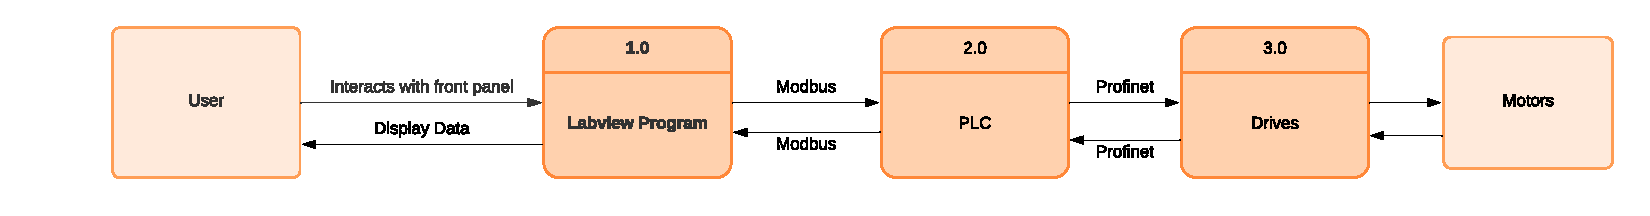
\includegraphics[width=0.75\columnwidth]{Pictures/DFD1.pdf}}
\caption{Dette nivå 1 \gls{dfdig} viser de tre hovedprosessene i programmet og hvordan dataen flytter mellom dem.}
\label{fig: lvl1}
\end{figure}
\begin{figure}[H]
\centerline{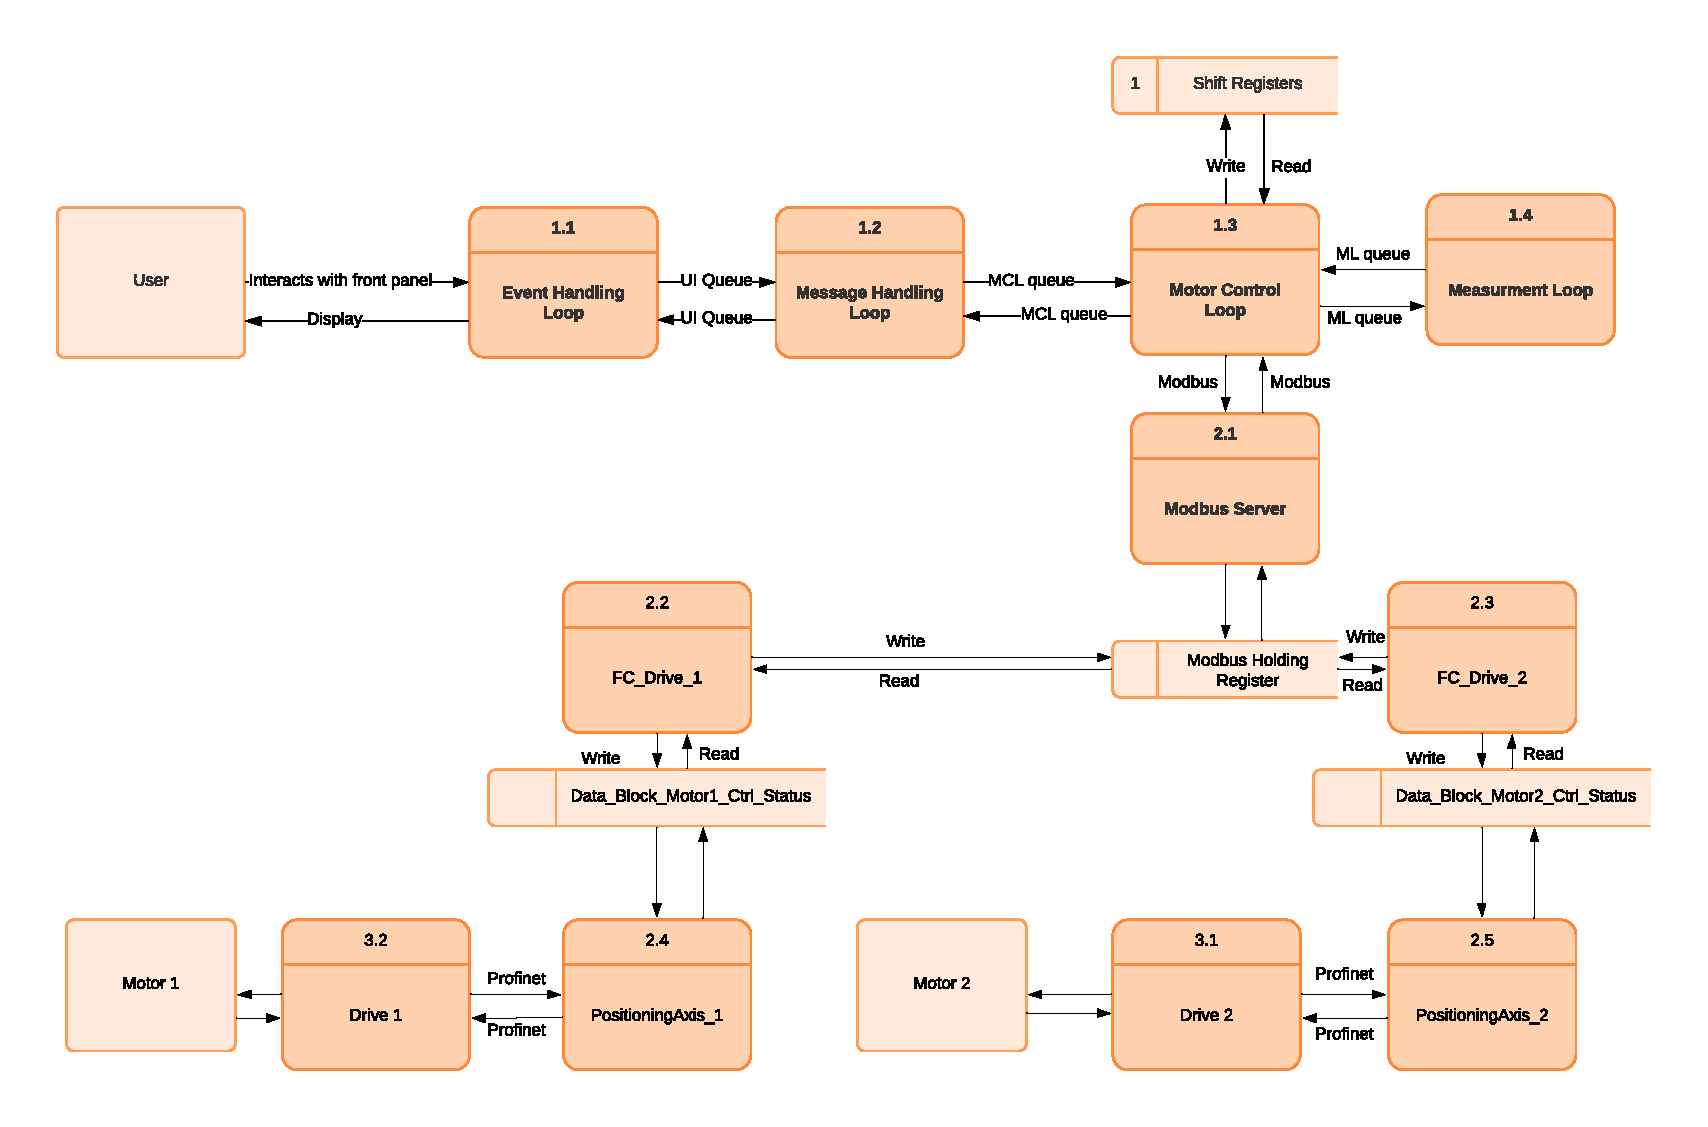
\includegraphics[width=0.75\columnwidth]{Pictures/DFD2.pdf}}
\caption{Dette nivå 2 \acrshort{dfd} viser de tre hovedprosessene i programmet og hvordan dataen flytter mellom dem med litt mer detalj enn i \figref{fig: lvl1}.}
\label{fig: lvl2}
\end{figure}
\subsection{Labview}
På klientsiden(PC) er koden skrevet i LabVIEW, spesifikt 2024 32-bit versjonen. Valget av denne versjonen ble gjort fordi ikke alle nødvendige moduler var tilgjengelige i 64-bit versjonen. For designet ble \acrfull{qmh}-designmønsteret valgt for å tillate samtidig datainnsamling, motorstyring og oppdateringer til brukergrensesnittet.
\subsubsection{Programstruktur}
 I denne seksjonen vil de forskjellige elementene i programmet bli beskrevet. Hvis en endring i et skiftregister ikke er nevnt, antar man at det er uendret fra forrige iterasjon. Programmet består av fire parallelle løkker: \acrlong{ehl}, \acrlong{mhl}, \acrlong{mcl} og \acrlong{ml}. De tre sistnevnte har sine egne køer som dataene flyter gjennom. Mesteparten av koden kjøres inne i løkkene, bortsett fra initialisering av køene i \acrshort{mhl}, initialisering av \gls{modbus}-tilkoblingen i \acrshort{mcl} og initialisering av tilkoblingen til forsterkeren i \acrshort{ml}.
\subsubsection*{''Event Handling''- Loop}

\begin{enumerate}[label={[\arabic*]}]
  \item \textbf{''Start'': Value Change}: Merker en endring i tilstanden til start-knappen på \glset{bg} og sender''Start''-meldingen til \acrshort{mhl}.
  \item \textbf{''Mode'': Value Change}: Merker en endring i tilstanden til mode-knappen på \glset{bg} og sender''mode''-meldingen sammen ved den valgte modusen til \acrshort{mhl}. Denne knappen er deaktivert etter at den blir trykket på slik at man ikke kan endre modus under kjøring.
  \item \textbf{"Reset'': Value Change}: Merker en endring i tilstanden til reset-knappen på \glset{bg} og sender''Reset''-meldingen til \acrshort{mhl} dette reaktiverer også mode-knappen på \glset{bg}.
  \item \textbf{''Setpoint Speed'': Value Change}: Merker en endring i tilstanden til ''Speed''-kontrollen på \glset{bg} og sender ''Speed''-meldingen til \acrshort{mhl} sammen med verdien valgt av brukeren. 
  \item \textbf{''Setpoint Torque'': Value Change}:  Merker en endring i tilstanden til ''Torque''-kontrollen på \glset{bg} og sender ''Torque''-meldingen til \acrshort{mhl} sammen med verdien valgt av brukeren. 
  \item \textbf{Panel Close?}: Merker om brukeren lukker frontpanelet og sender ''Confirm Quit''-meldingen til \acrshort{mhl}.
  \item \textbf{Application Instance Close}: Ikke tatt i bruk.
  \item \textbf{Timeout}: Hvis ingen endringer på \glset{bg} merkes innen $200ms$ aktiveres denne ''casen' og sender ''Update''-meldingen til \acrshort{mhl}.
  \item \textbf{''Exit''}: Merker en endring i tilstanden til Exit-knappen på \glset{bg} og sender''Exit''-meldingen til \acrshort{mhl}.
 \item \textbf{''Stop'': Value Change}: Merker en endring i tilstanden til stop-knappen på \glset{bg} og sender''stop''-meldingen til \acrshort{mhl} dette reaktiverer også mode-knappen på \glset{bg}.
 \item \textbf{''Emergency Stop'': Value Change}: Merker en endring i tilstanden til ''Emergency Stop''-knappen på \glset{bg} og sender''E-stop''-meldingen til \acrshort{mhl} dette reaktiverer også mode-knappen på \glset{bg}.
 \item \textbf{<User Event - Stop>: User Event}: Håndterer andre stop hendelser fra \glset{bg}.
\end{enumerate}

\subsubsection*{''Message Handling'' - Loop}

\begin{itemize}
    \item \textbf{Init}: Ved oppstart mottar \acrfull{mhl}, \acrfull{mcl} og \acrfull{ml}-loopene ''Init''-meldingen fra \textit{Create All Message Queues.vi} denne VI-en lager også køene de ulike loopene bruker. Referansene til front panelet blir initialisert.''Update Display'' blir sendt tilbake til \acrshort{mhl} med verdien ''Initializing System''
    \item \textbf{Update Display:}Verdien sendt sammen med ''Update Display''-meldingen blir konvert til \gls{str} og blir fremvist i ''Status''-indikatoren på frontpanelet.
    \item \textbf{Mode:} Videresender den valgte modusen til \acrlong{mcl}
    \item \textbf{Reset:} Videresender ''Reset''-meldingen til \acrshort{mcl}
    \item \textbf{Ok:} Når ''OK''-meldingen blir mottatt fra \acrshort{mcl} som betyr at kommunikasjon med begge drivene har blitt etablertsatt ter den et \glssk{bool} flagg til \true. Når dette flagget er \false stopper det \acrshort{mhl} fra å sende flere ''Update''-meldinger til \acrshort{mcl}. 
    \item \textbf{Update:} Dersom ''Ok'' flaget sattsendes en ''Update''-melding til \acrshort{mcl}, hvis ikke gjør den ingen ting.
    \item \textbf{Speed:} Sender ''Update Display''-melding med verdien ''Starting Motor control'' til \acrshort{mhl}-køen og sender ''Set speed''-meldingen til \acrshort{mcl} med den mottatte fartsverdien. 
    \item \textbf{Torque:} Sender ''Update Display''-melding med verdien ''Torque Changed'' til \acrshort{mhl}-køen og sender ''Set torque''-meldingen til \acrshort{mcl} med den mottatte momentverdien. 
    \item \textbf{Stop:} Sender ''Update Display''-melding med verdien ''Stopping Motors'' til \acrshort{mhl}-køen og sender ''Stop''-meldingen til \acrshort{mcl} med prioritet. 
    \item \textbf{E-Stop:} Sender ''Update Display''-melding med verdien ''Emergency Stop, reset required til continue'' til \acrshort{mhl}-køen og sender ''E-Stop''-meldingen til \acrshort{mcl} med prioritet. 
    \item \textbf{Start:} Sender ''Update Display''-melding med verdien ''Starting'' til \acrshort{mhl}-køen og sender ''Start''-meldingen til \acrshort{mcl}. 
    \item \textbf{Error:} Håndterer den mottatte feilen ved hjelp av \textit{Simple Error Handler.vi} og sender ''Update Display''-meldingen sammen med en beskrivelse av feilen til \acrshort{mhl}.   
    \item \textbf{Confirm Quit:} Sender ''Exit''-meldingen til \acrshort{mhl} med prioritet. 
    \item \textbf{Exit:} Frigjør referansen til \acrshort{ui}-køen og sender ''Exit''-meldingen til \acrshort{mcl} og \acrshort{ml}.
    \item \textbf{Default:} Håndterer udefinerte meldinger til \acrshort{mhl} med å kaste en feilmelding. 
\end{itemize}
\textbf{Motor Control Loop}
\begin{itemize}
    \item \textbf{Init:} Setter de \glspl{boolean} til registret(som vist i \figref{fig:MotorBoolCl}) til \false ogsatt tpunktene til fart og moment til $0$.  Write \glsen{bool} blir satt til \true for å tillate verdiene til å bli sendt via \gls{modbus}-tilkoblingen. Sender ''Update Display''-meldingen med verdien ''Initialising Motors'' til \acrshort{mhl}-køen. 
    \item \textbf{Modes:} Tar den valgte modusen og konverterer den fra \gls{var} til \gls{bool}  ogsatt ter ''Mode''-flagg skiftregisteret.
    \item \textbf{Reset:} Sender ''Stop''-meldingen med prioritet og ''Init''-melding til \acrshort{mcl}. Den sender også ''Reset''-meldingne til \acrlong{ml}.
    \item \textbf{Update:} Sender ''Update''-meldingen til \acrshort{ml}. Hvis Asynchronus-modus er aktivertsatt ter kontrolleren et nyttsatt tpunkt på farten til motor 2. Skriving over modbus slås på og verdiene 
 i registeret sendes.
    \item \textbf{Set Speed:} Tar den mottatte fartsverdien og konverterer den fra  \gls{var} til \gls{dbl}, lagrer den i skifteregister ''Setpoint Speed'' ogsatt ter "write"-flagg skiftregisteret til \true. 
    \item \textbf{Set Torque:} Tar den mottatte momentverdien og konverterer den fra  \gls{var} til \gls{dbl}, lagrer den i skifteregister ''Setpoint Torque'' ogsatt ter ''write''-flagg skiftregisteret til \true. 
    \item \textbf{Get Torque:}  Tar den mottatte momentsverdien fra \acrshort{ml} og konverterer den fra \gls{var} til \gls{dbl}, lagrer den i skiftregisteret ''Measured Torque'' og viser den på frontpanelet.
    \item \textbf{Stop:} Setter de \glspl{boolean} ''StartMotor1'' og ''StartMotor2''  til \false samt ''Write'' og''MotorsOff'' til \true. Farts- og momentsettpunktenesatt tes til $0$. ''Stop''-meldingen blir sent til loggeloopen med prioritet.
      \item \textbf{E-Stop:} Setter de \glspl{boolean} ''StartMotor1'', ''StartMotor2'' og ''MotorsOff'' til \false samt ''Write'' og''E-stop'' til \true. Farts- og momentsettpunktenesatt tes til $0$. ''Stop''-meldingen blir sent til loggeloopen med prioritet.
    \item \textbf{Start:}  Sender ''Logging''-meldingen til \acrshort{ml} ogsatt ter de \glssk{boolean} ''StartMotor1'', ''StartMotor2'' og  ''Write'' til  \true. ''MotorsOff'' blir satt til \false. 
    \item \textbf{Exit:} Frigjør referansen til \acrshort{mcl}-køen og sender ''Exit''-meldingen til \acrshort{ml}.Setter også motorkontrollverdiene til enten $0$ eller \false med unntak av ''Stop''-variablen som blir satt til {\true}. Håndterer eventuelle gjenstående feilmeldinger ved hjelp av \textit{SimpleErrorhandler.vi}
    \item \textbf{Default:} Håndterer eventuelle udefinerte meldinger mest i utviklings- og feilsøkingsfasene.
\end{itemize}

\textbf{Measurement loop}
\begin{itemize}
    \item \textbf{Init:} Sender meldingen ''Update Display'' til \acrshort{mhl} med verdien ''Initializing Sensor''. Et \glssk{bool} flagg blir satt til \true. 
    \item \textbf{Update:} Sender meldingen ''Get Torque'' til \acrshort{mcl} med den målte momentverdien. Hvis det \glsske{bool} flagget fra ''Init''-casen er \true sender den meldingen ''Update Display'' til \acrshort{mhl} med verdien ''Sensor Initialized'' det \glsske{bool} flaggetsatt tes så til \false. 
    \item \textbf{Exit:} Frigjør referansen til \acrshort{ml}-køen. Håndterer eventuelle gjenstående feilmeldinger ved hjelp av \textit{SimpleErrorhandler.vi}
    \item \textbf{Default:} Ubrukt
\end{itemize}

\subsection{PLS-programmering}
Programvaren på \acrshort{pls}-siden som er en \Gls{s71500} er i hovedsak laget i \acrshort{fbd}, men også noe \acrshort{stl}. Under kjøring skifter ''Main Program Sweep'' gjennom 3 hovedfunksjonsblokker FC\_Drive 1, FC\_Drive 2 og MB\_SERVER hvor de til første kontrollerer henholdsvis drive 1 og 2, MB\_SERVER ER Modbus serveren som Klient PC-en kommuniserer med for å sende de ulike verdiene frem og tilbake. Et overblikk over denne Organisasjonsblokken(OB)  er vist i \figref{fig:OB1}. Modbus-serverblokken kommuniserer med klienten og mottar data. Denne dataen blir så lagret i en datablokk som vist i   \figref{fig:dbHoldReg}. De til funksjonsblokkene får aksesser datablokken stortsatt t uavhengig av hverandre, men noen variabler er delt slik som::
\begin{itemize}
    \item MotorsOn
    \item Reset
    \item MotorsOff
    \item Emergency Stop
\end{itemize}
Alle disse blir satt av klientet. 
De ikke-delte variablene er:
\begin{multicols}{2}
Motor 1
\begin{itemize}
    \item StartMotor1
    \item SetSpeed1Msb
    \item SetSpeed1lsb
    \item ReadSpeed1Msb
    \item ReadSpeed1lsb
    \item Motor1Ok
\end{itemize}
Motor 2 
\begin{itemize}
    \item StartMotor2
    \item SetSpeed2Msb
    \item SetSpeed2lsb
    \item ReadSpeed2Msb
    \item ReadSpeed2lsb
    \item Motor2Ok
\end{itemize}
\end{multicols}
For begge funskjonsblokkene gjelder det at de første 3 blir satt av klienten og de 3 siste blir satt av \acrshort{pls}. 
Det følgende er en forklaring av de ulike blokkene i FC\_Drive\_1  disse er identiske til FC\_Drive\_2 ved passende endring av variabler. 
\begin{enumerate}[label= \textbf{Network \arabic*:}]
    \item \textbf{ Motor\_1\_MC\_Power} Hvis Enable\_MC\_Power er \true blir motoren slått på, dersom det oppstår en feilmelding skriv den til Sts\_MC\_Error.
    \item \textbf{ Motor\_1\_MC\_Reset} Hvis Execute\_MC\_Reset er \true reset motoren.
    \item \textbf{ Motor\_1\_MC\_Halt} Hvis Execute\_MC\_Halt er  \true stans motoren.
    \item \textbf{ Motor\_1\_MC\_jog} Hvis Execute\_Jog\_Forward er  \true flytt motoren  fremover med farten satt av Sp\_lr\_Velocity. 
    
    Hvis {Execute\_Jog\_Backward\footnote{Ikke i bruk}} er  \true flytt motoren  bakover med farten satt av Sp\_lr\_Velocity. 
    \item \textbf{ Motor\_1\_MoveVelocity} Flytter motoren hvis Execute er  \true, Man kansatt te  Velocity, Acceleration, Deceleration, Jerk og  Direction slik man ønsker\footnote{Denne blokken ble brukt i starten av utviklingen av programmet, men å endre fart under kjøring viste seg å være komplisert derfor ble MC\_Jog brukt isteden}.  
    \item \textbf{Motor\_1\_Home}\footnote{Siden vi ikke gjør posisjonskontroll så bryr vi oss ikke hvor motoren tror den er ved oppstart. Funksjonen er lagt i programmet for eventuelt endring av bruksområde i fremtiden.} Hvis Execute\_MC\_Home er  \true start homing av motoren .
    \item \textbf{Motor\_1\_Stop} hvis Execute\_MC\_Stop er  \true stop motoren, Dette er forskjellig fra MC\_Halt ved at vi låser aksen slik at om den mottar nye ''Motion Commands'' vil den ikke bevege seg. Før den blir resatt. Denne brukes stil å realisere programstyrt nødstopp.
    \item \textbf{Motor 1 actual velocity} Leser av hastighetsverdien fra posisjonsaksen og flytter den til lr\_Actual\_Velocity-variabelen.
    \item \textbf{Motor 1 Actual Torque}\footnote{Ubrukt} Leser av momentverdien fra posisjonsaksen og flytter den til lr\_Actual\_Torque-variabelen.
    \item \textbf{Motor 1 Torque Range}\footnote{For å bruke denne funksjonen må man bruke telegram 750, dette telegrammet tror jeg ikke \Gls{s71500} er kompatibel med. Denne funskjonen er derfor ikke i bruk.}  Hvis Enable\_Torque\_Reduction er  \true begrenser den driven til området satt av  Sp\_lr\_Torque\_Lower\_Limit og Sp\_lr\_Torque\_Upper\_Limit.
    \item \textbf{Read Velocity Motor 1} Tar lr\_Actual\_Velocity variabelen som er en \Gls{lreal} og splitter den til to \gls{word} til bruk i \gls{modbus}-kommunikasjonen. Et mer detaljert bilde av funksjonaliteten er vist i \figref{fig:split}.
    \item \textbf{Turn on Motor 1} Hvis $MotorRegisters[0] = 1$ blir Enable\_MC\_Power satt  til \true. Hvis $MotorRegisters[0] = 0$ blir Enable\_MC\_Power satt  til \false. Detaljene er vist i \figref{fig:WTB}.
    \item \textbf{Stop Motors} Hvis $MotorRegisters[8] = 1$ blir Execute\_MC\_Halt satt  til \true. Hvis $MotorRegisters[8] = 0$ blir Execute\_MC\_Halt satt til \false. Detaljene er vist i \figref{fig:WTB}.
    \item \textbf{Set Speed} Spleiser High og Low \glspl{word}  over \gls{modbus} sammen til en \Gls{lreal} og flytter den til Sp\_lr\_Velocity-variabelen. Detaljene er vist i \figref{fig:Splice}.
    \item \textbf{Move Jog} Hvis $MotorRegisters[2] = 1$ blir Execute\_Jog\_Forward satt  til \true. Hvis $MotorRegisters[2] = 0$ blir Execute\_Jog\_Forward satt til \false. Detaljene er vist i \figref{fig:WTB}.
    \item \textbf{Motor Status Flag} Hvis $Sts\_MC\_Error = \true $ eller $Enable\_MC\_Power \neq \true$ blir $MotorRegisters[13]=0$ hvis ikke blir den satt til $1$. Detaljene er vist i Kode \ref{lst:MotorStatus}.
    \item \textbf{Motor 1 Reset} Hvis $MotorRegisters[1] = 1$ blir Execute\_MC\_Reset satt til \true. Hvis $MotorRegisters[1] = 0$ blir Execute\_MC\_Reset satt til \false. Detaljene er vist i \figref{fig:WTB}.
    \item \textbf{Execute Emergency Stop} Hvis $MotorRegisters[15] = 1$ blir Execute\_MC\_Stop satt til \true. Hvis $MotorRegisters[1] = 0$ blir Execute\_MC\_Stop satt til \false. En resett er påkrevd for at motoren vil akseptere nye ''motion commands''. Detaljene er vist i \figref{fig:WTB}.
\end{enumerate}
\clearpage
\appendix

\addcontentsline{toc}{section}{Ordliste}
\addcontentsline{toc}{subsection}{Akronymer}
\printglossary[type=\acronymtype]
\newacronym{qmh}{QMH}{Queued Message Handler}
\newacronym{ehl}{EHL}{Event Handling Loop}
\newacronym{mhl}{MHL}{Message Handling Loop}
\newacronym{mcl}{MCL}{Motor Control Loop}
\newacronym{ml}{ML}{Measurement loop}
\newacronym{ui}{UI}{User Interface, se \gls{bg}}
\newacronym{pls}{PLS}{Programmerbar logisk styring}
\newacronym{tia}{TIA}{Totally Integrated Automation}
\newacronym{fbd}{FBD}{Funksjonsblokkdiagram}
\newacronym{dfd}{DFD}{Dataflytdiagram, se \gls{dfdig}}
\newacronym{stl}{STL}{Strukturert tekst}
\addcontentsline{toc}{subsection}{Begreper}
\printglossary
\newglossaryentry{vi}{
name = {vi},
description = {står for ''Virtual Instrument''. Det er et program eller en subrutine skrevet i LabVIEW.}
}
\newglossaryentry{var}{
  name={variant},
  description={I LabVIEW er variant-datatypen en fleksibel variabel som kan inneholde hvilken som helst type data. I \acrlong{qmh} sendes all data som varianter}
}
\newglossaryentry{type}{
name = {typedef},
description ={I LabVIEW er en Type Definisjon en tilpasset kontroll eller indikator som lagres som en egen fil med en .ctl-utvidelse. Dette lar deg definere en datatype én gang og bruke den på tvers av flere \Gls{vi}s. Når du oppdaterer Typedef, oppdateres alle instanser av den automatisk, noe som sikrer konsistens.}
}
\newglossaryentry{str}{
name = {streng},
description = {Datatype som refererer til en sekvens av tegn, vangligvis tekst. Kan inneholde bokstaver, tall, symboler og mellomrom}
}
\newglossaryentry{boolean}{
  name={boolsk verdi},
  description={ Bolske verdier kan holde til mulige verdier : \true eller \false alternativt $0$ eller $1$},
  plural = {bolske verdiene}
}
\newglossaryentry{bool}{
  name={bool},
  description={see \gls{boolean}},
  sk = {boolsk},
  ske = {boolske},
  en = {boolen}
}
\newglossaryentry{dbl}{
  name={double},
  description={en numerisk datatype med dobbel presisjon for flyttall (64 biter i størrelse}
}
\newglossaryentry{word}{
  name={word},
  plural={word-ene},
  description={et binært tall uten fortegn som representerer en numerisk heltallsdatatype (16 bit i størrelse)}
}
\newglossaryentry{real}{
  name={Real},
  description={et 32-bits \gls{flt}}
}
\newglossaryentry{flt}{
name = {flyttall},
description = {Flyttall er tall uttrykt ved hjelp av en desimalbrøk og en eksponent. De brukes i datamaskiner for å representere reelle tall}
}
\newglossaryentry{bg}{
name = {brukergrensesnitt},
et = {brukergrensesnittet},
description = {Et brukergrensesnitt er kontaktpunktet mellom brukeren og et system, som for eksempel et operativsystem, programmer eller nettsider. Består som oftest av ikoner, knapper, vinduer osv...}
}

\newglossaryentry{lreal}{
  name={LReal},
  description={I Siemens \Gls{step7} er LREAL datatypen “Long Real” og et 64-bit flyttall}
}
\newglossaryentry{step7}{
  name={Step 7},
  description={Step 7 er et programvareverktøy utviklet av Siemens for å programmere og konfigurere deres \acrshort{pls}. Det er en del av \acrshort{tia}-portalen, som er et miljø for automatisering}
}
\newglossaryentry{modbus}{
name ={modbus},
description={er en kommunikasjonsprotokoll for bruk i \acrlong{pls}}
}
\newglossaryentry{s71500}{
name = {S7-1500},
description={SIMATIC S7-1500, CPU 1511-1 PN, sentral prosesseringenhet med arbeidsminne på 150 KB for program og 1 MB for data, 1. grensesnitt: PROFINET IRT med 2-port switch, 60 ns bit-ytelse, SIMATIC minnekort er nødvendig. \url{https://mall.industry.siemens.com/mall/en/ww/catalog/product/6es7511-1ak02-0ab0}}
}
\newglossaryentry{dfdig}{
name = {Dataflytdiagram},
description = {Denne typen diagram viser hvordan data beveger seg gjennom et system, inkludert kilder, destinasjoner og lagringspunkter. Det kan brukes på forskjellige nivåer fra $0$ til $3$, hvor hvert nivå har et økende detaljnivå.}
}
\section{''Strukturert tekst''-programmering} 


\begin{lstlisting}[language=ST,caption={Setting Motor Status},label={lst:MotorStatus}]
IF 
    "Data_block_Motor1_Ctrl_Status".Structure_Drive_2.Sts_MC_Error 
OR 
NOT  
    ("Data_block_Motor1_Ctrl_Status".Structure_Drive_2.Enable_MC_Power) 
    THEN
        "dbHoldingRegisters".MotorRegisters[14] := 0;
ELSE
    "dbHoldingRegisters".MotorRegisters[14] := 1;
END_IF;

\end{lstlisting}
\begin{lstlisting}[language=ST,caption={Attempt at changing velocity when using the MC\_Move\_Velocity. In the end it was more efficient to use MC\_Move\_Jog instead},label={lst:Vel}]
IF "Data_block_Motor1_Ctrl_Status".Structure_Drive_2.Sp_lr_Velocity <> #SetPoint THEN
    // SetPoint Changed': 'Clear' execution
    "Data_block_Motor1_Ctrl_Status".Structure_Drive_2.Execute_MC_Velocity:=FALSE;
ELSE
    "Data_block_Motor1_Ctrl_Status".Structure_Drive_2.Sp_lr_Velocity := #SetPoint;
    "Data_block_Motor1_Ctrl_Status".Structure_Drive_2.Execute_MC_Velocity := TRUE;
END_IF;
\end{lstlisting}




\section{''Function Block''-diagrammer}

\begin{figure}[H]
    \centering
    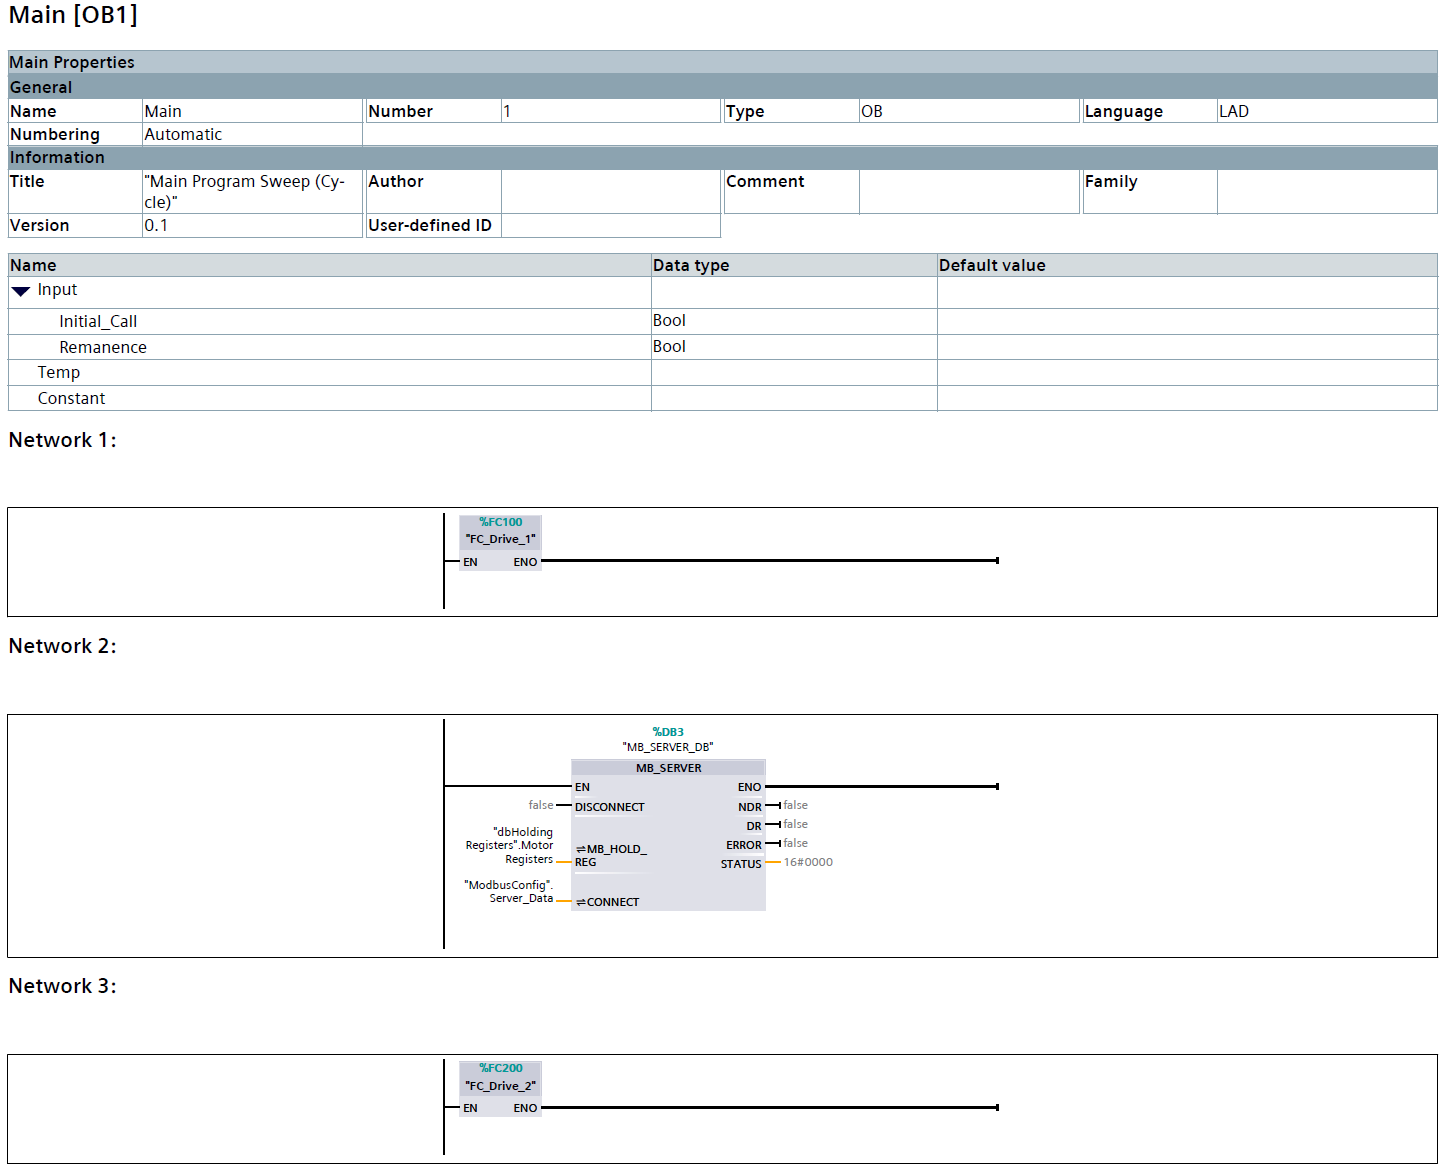
\includegraphics[width=0.5\linewidth]{FBDs/MainProgramSweep.PNG}
    \caption{''Main Program Sweep cycle'' på \acrshort{pls}-en.}
    \label{fig:OB1}
\end{figure}


\newgeometry{scale=0.75}
\thispagestyle{empty}
{%
\begin{figure}[H]
    \centering
    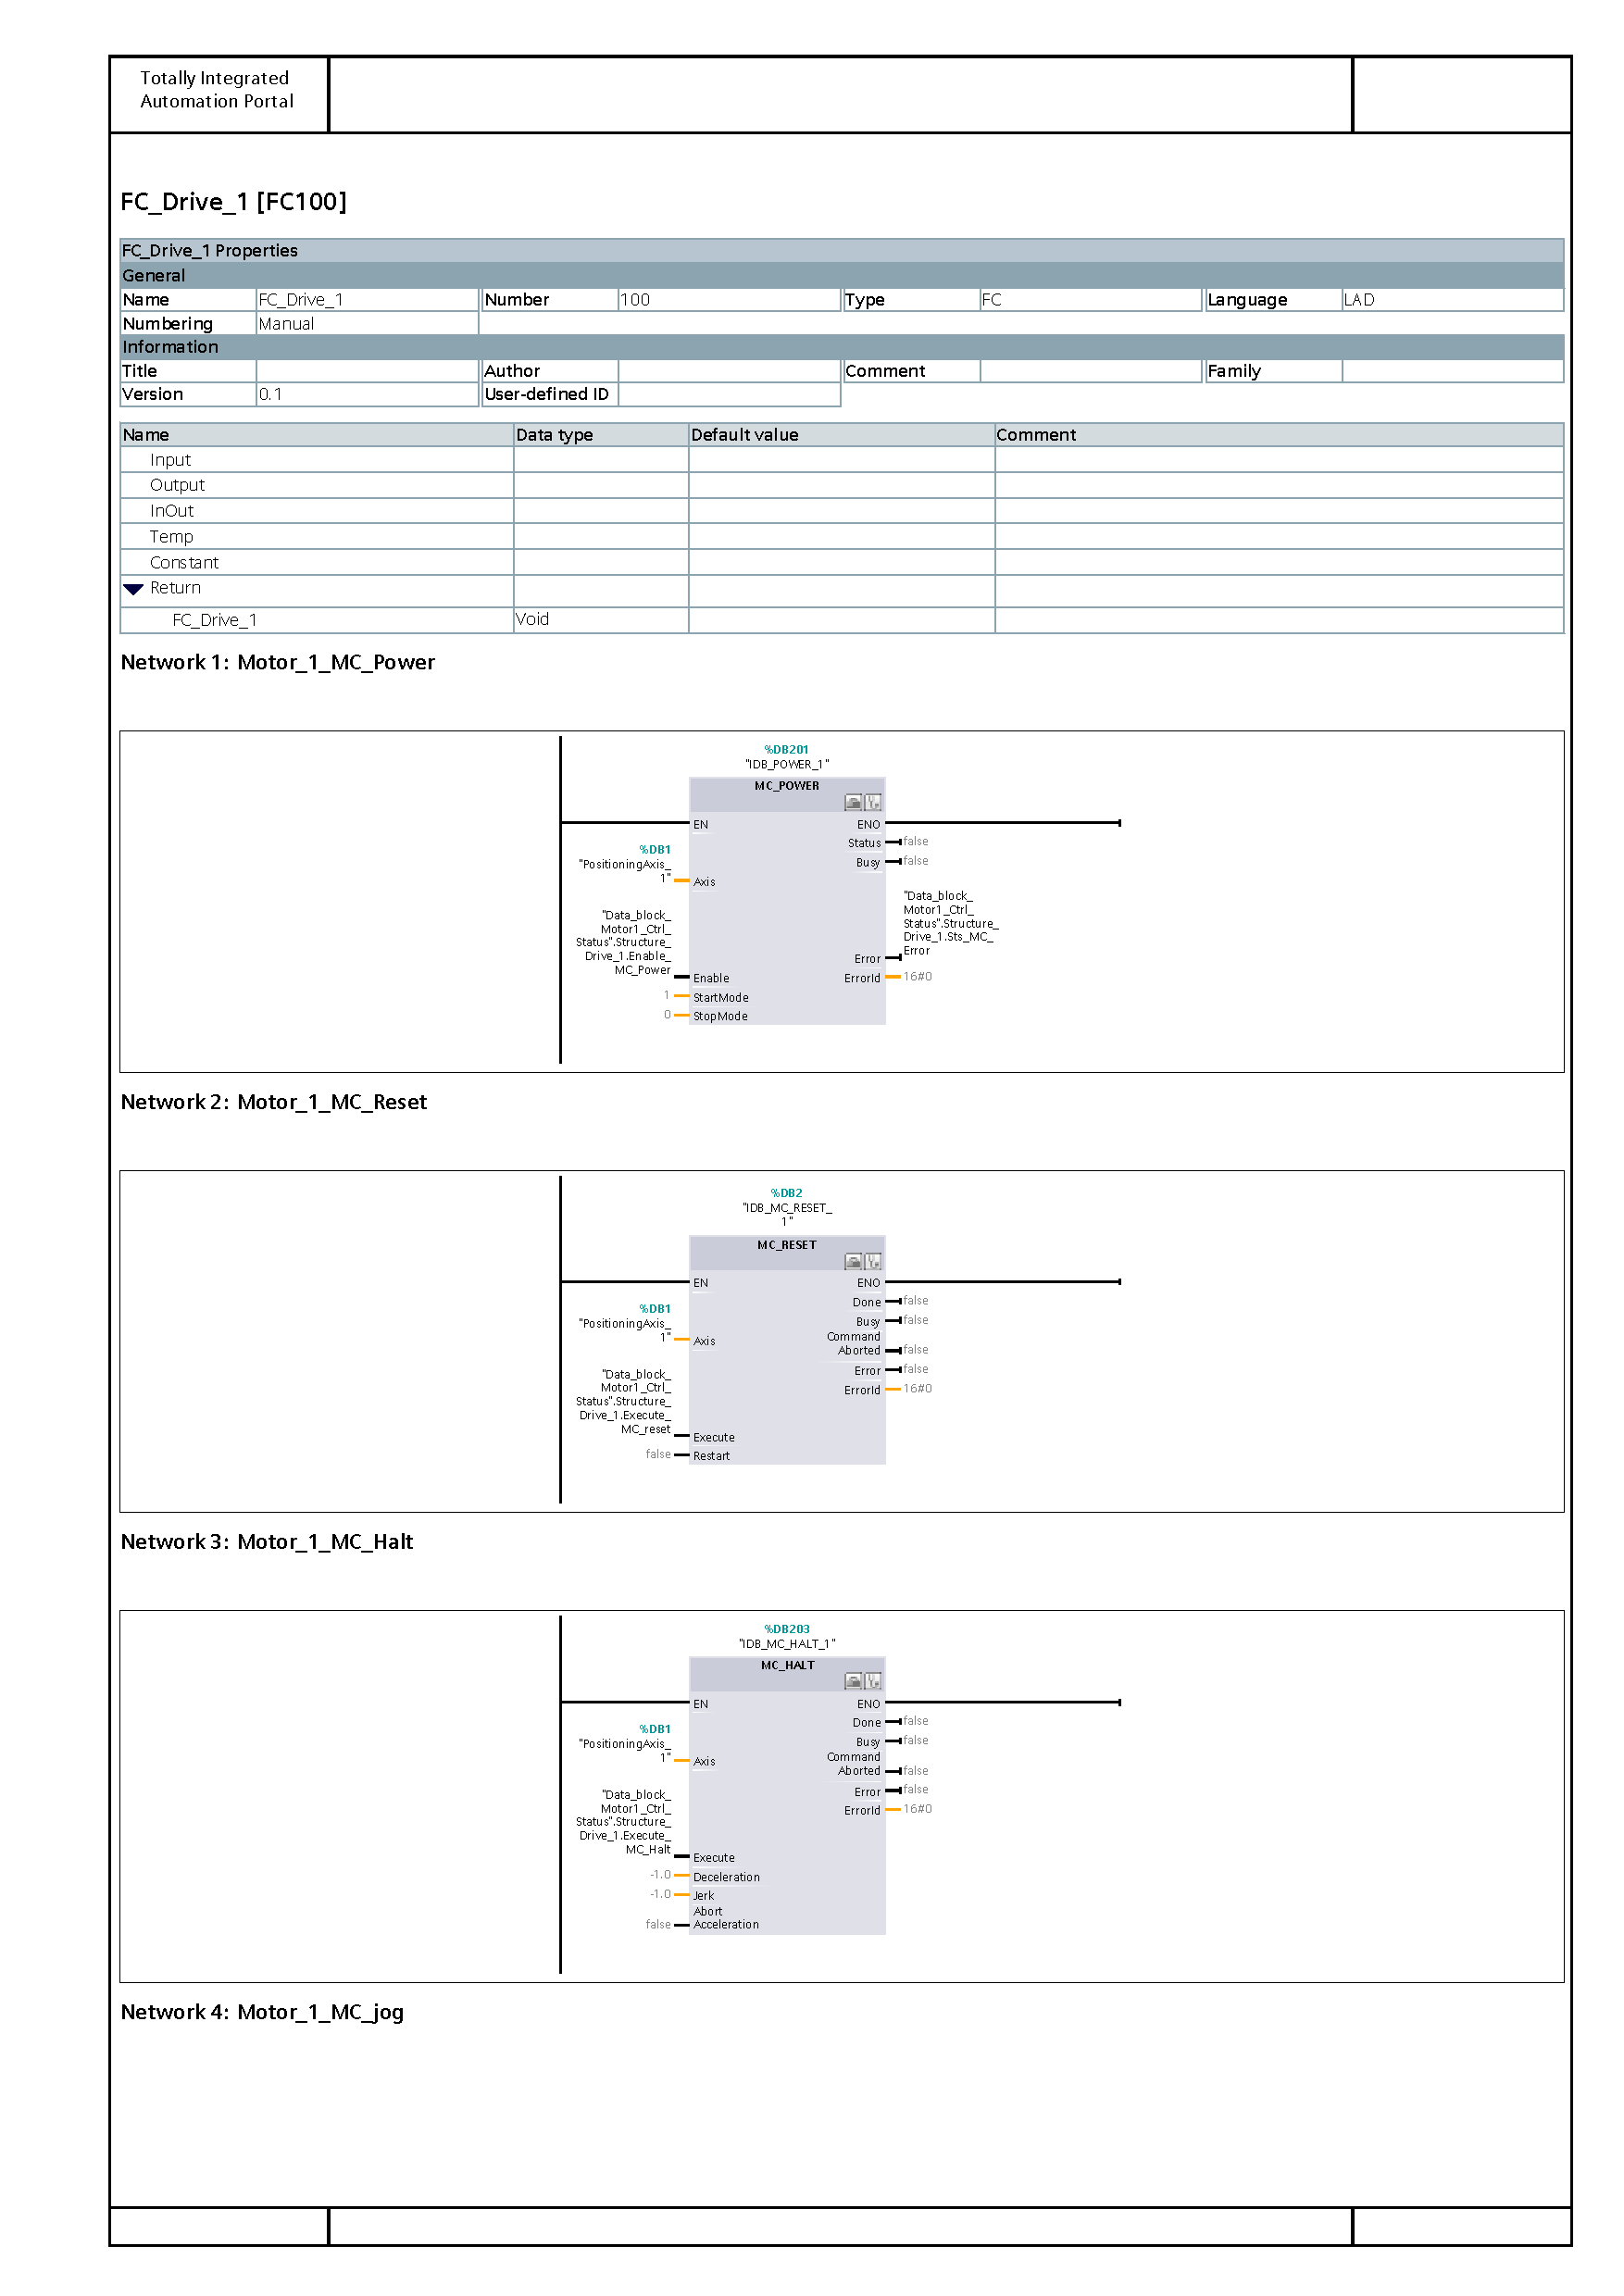
\includegraphics[page=1,scale=.5]{FBDs/FC_1.pdf}
    \caption{Funksjonsblokken som styrer Drive 1,  funksjonsblokk for Drive 2 lik med passende endring av variabler.}
    \label{fig:FC1}
\end{figure}
  \par
}
\includepdf[pages={2-4},scale=.75]{FBDs/FC_1.pdf}
\restoregeometry

\begin{figure}[H]
    \centering
    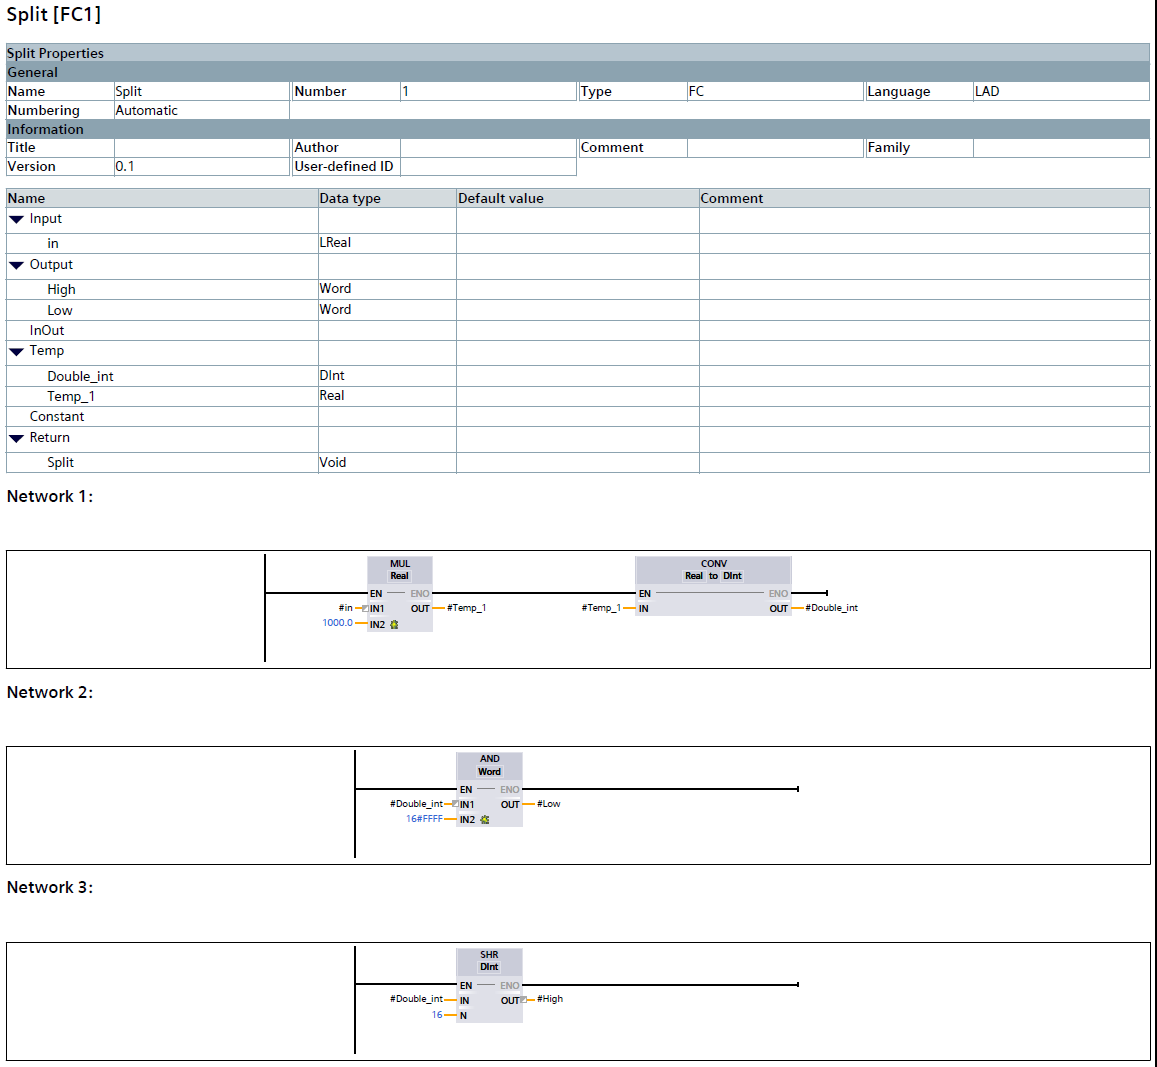
\includegraphics[width=0.5\linewidth]{FBDs/split.PNG}
    \caption{Funksjonsblokk for splitting av en 64-bit \Gls{lreal} til to 16-bit \gls{word}}
    \label{fig:split}
\end{figure}
\begin{figure}[H]
    \centering
    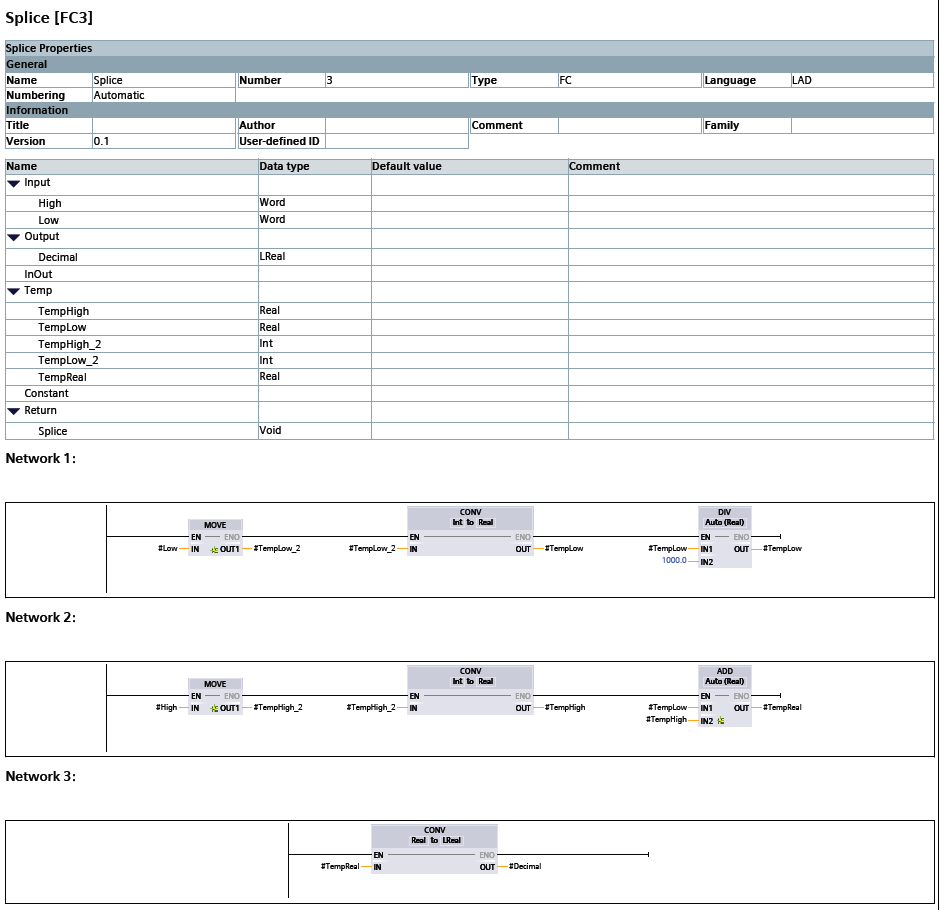
\includegraphics[width=0.5\linewidth]{FBDs/Splice.PNG}
    \caption{Funksjonsblokk for å spleise sammen en 32-bit \Gls{real}(flyttall) fra to 16 bit \glspl{word} før denne konverteres til en 64 bit \Gls{lreal}.}
    \label{fig:Splice}
\end{figure}

\begin{figure}[H]
    \centering
    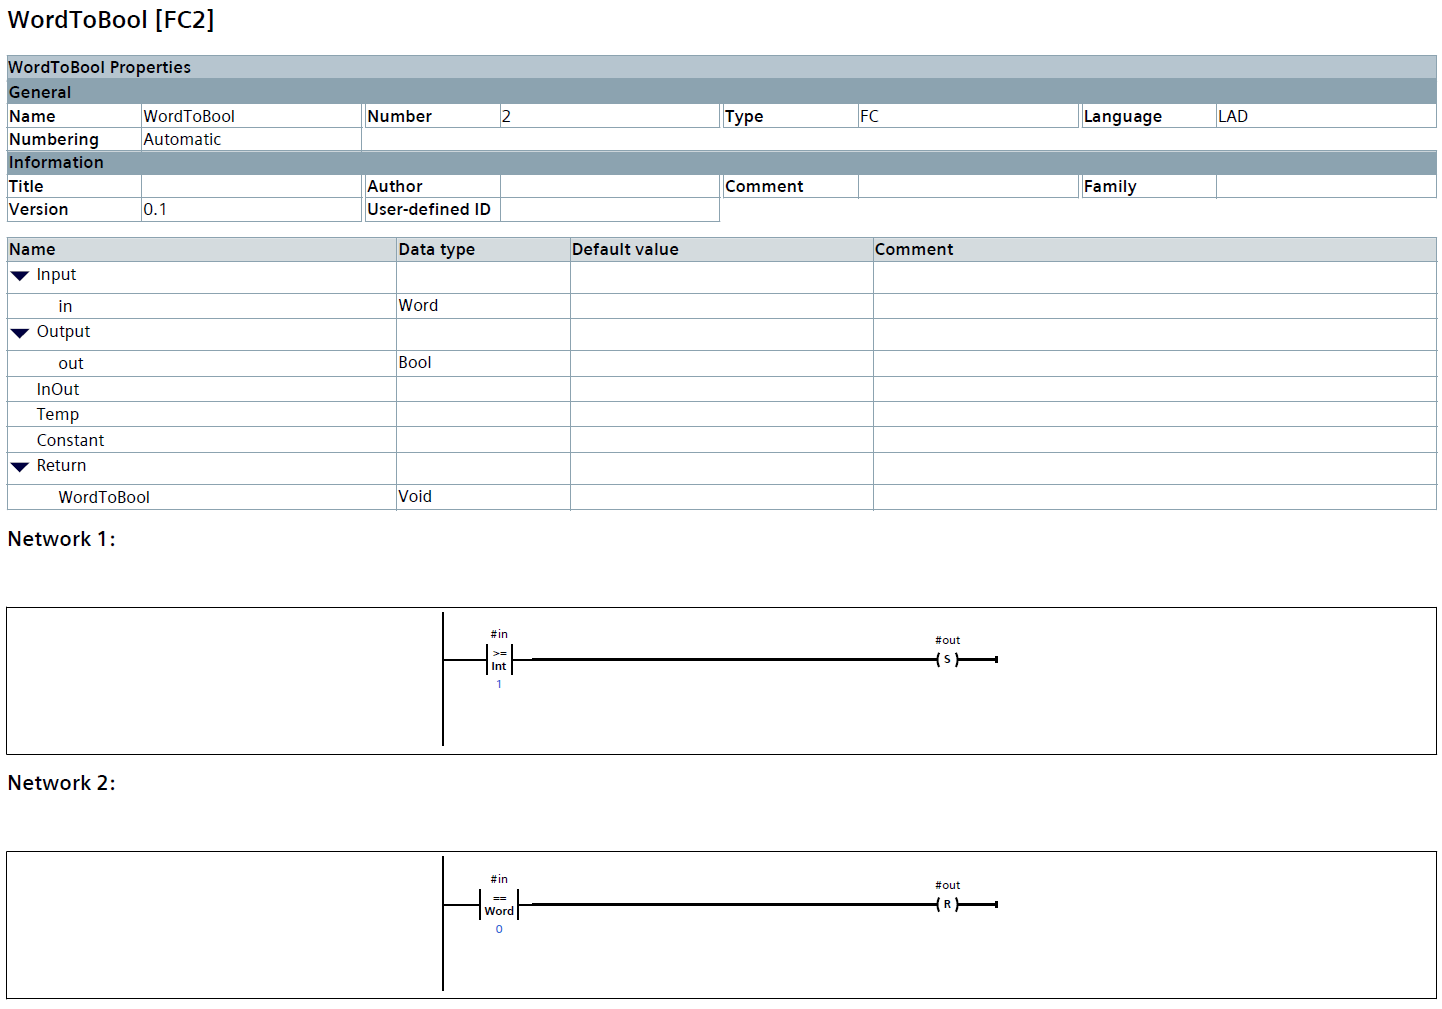
\includegraphics[width=0.5\linewidth]{FBDs/WordToBool.PNG}
    \caption{Funksjonsblokk for å konvertere et 16-bit \gls{word}(som kun tar veriene $0$  eller  $1$) til en 1-bit \glssk{bool} verdi}
    \label{fig:WTB}
\end{figure}
\section{Data Blocks}
\begin{figure}[H]
    \centering
    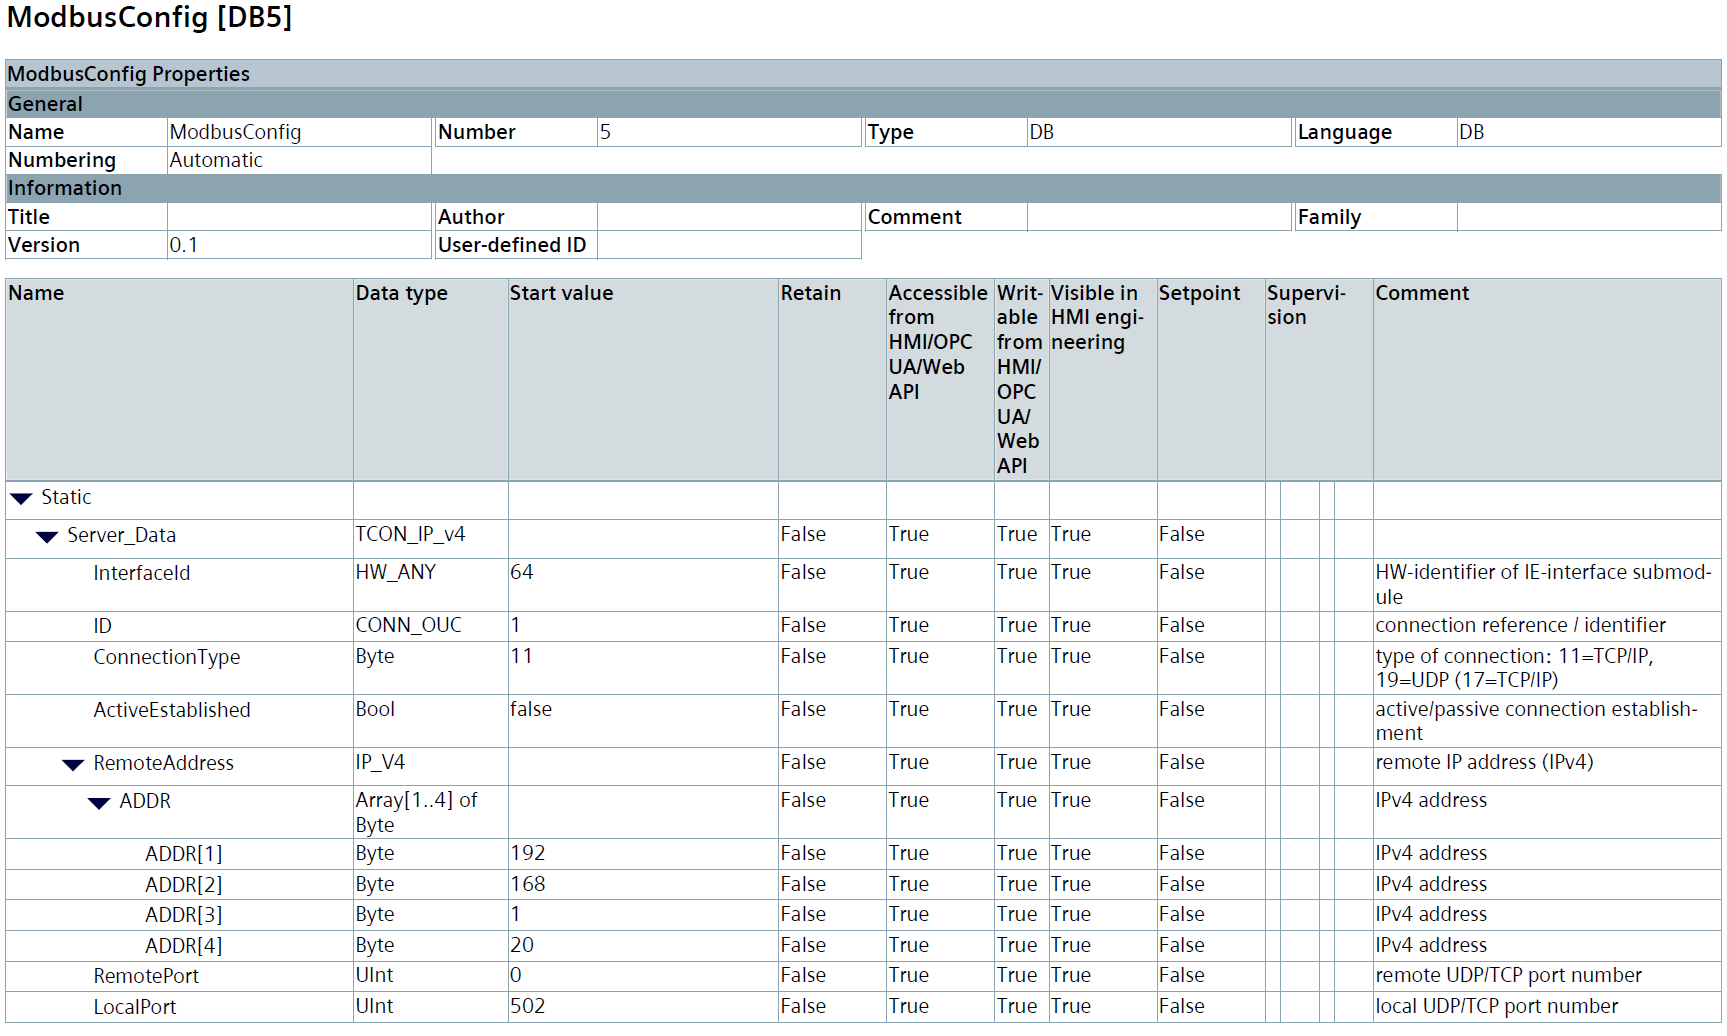
\includegraphics[width=0.5\linewidth]{DBs/ModbusConfig.PNG}
    \caption{Datablokk  som setter opp Mobus-Serveren på \acrshort{pls}-en.}
    \label{fig:ModbusConfig}
\end{figure}
\begin{figure}[H]
    \centering
    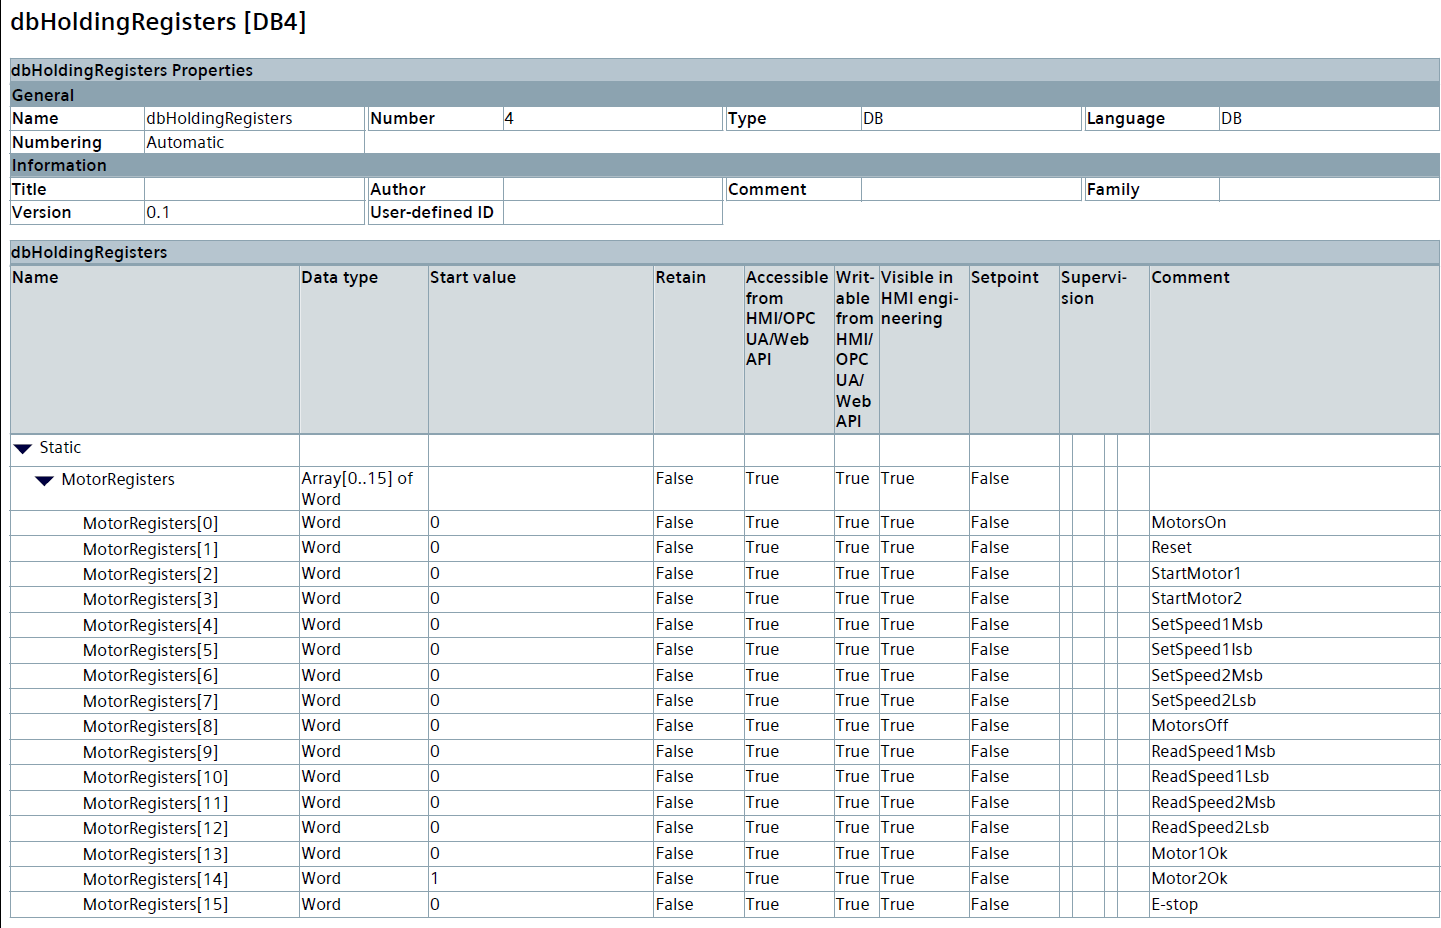
\includegraphics[width=0.5\linewidth]{DBs/dbHoldingRegisters.PNG}
    \caption{Datablokk med de ulike registrene sent frem og tilbake over Modbus-tilkoblingen.}
    \label{fig:dbHoldReg}
\end{figure}
\begin{figure}[H]
    \centering
    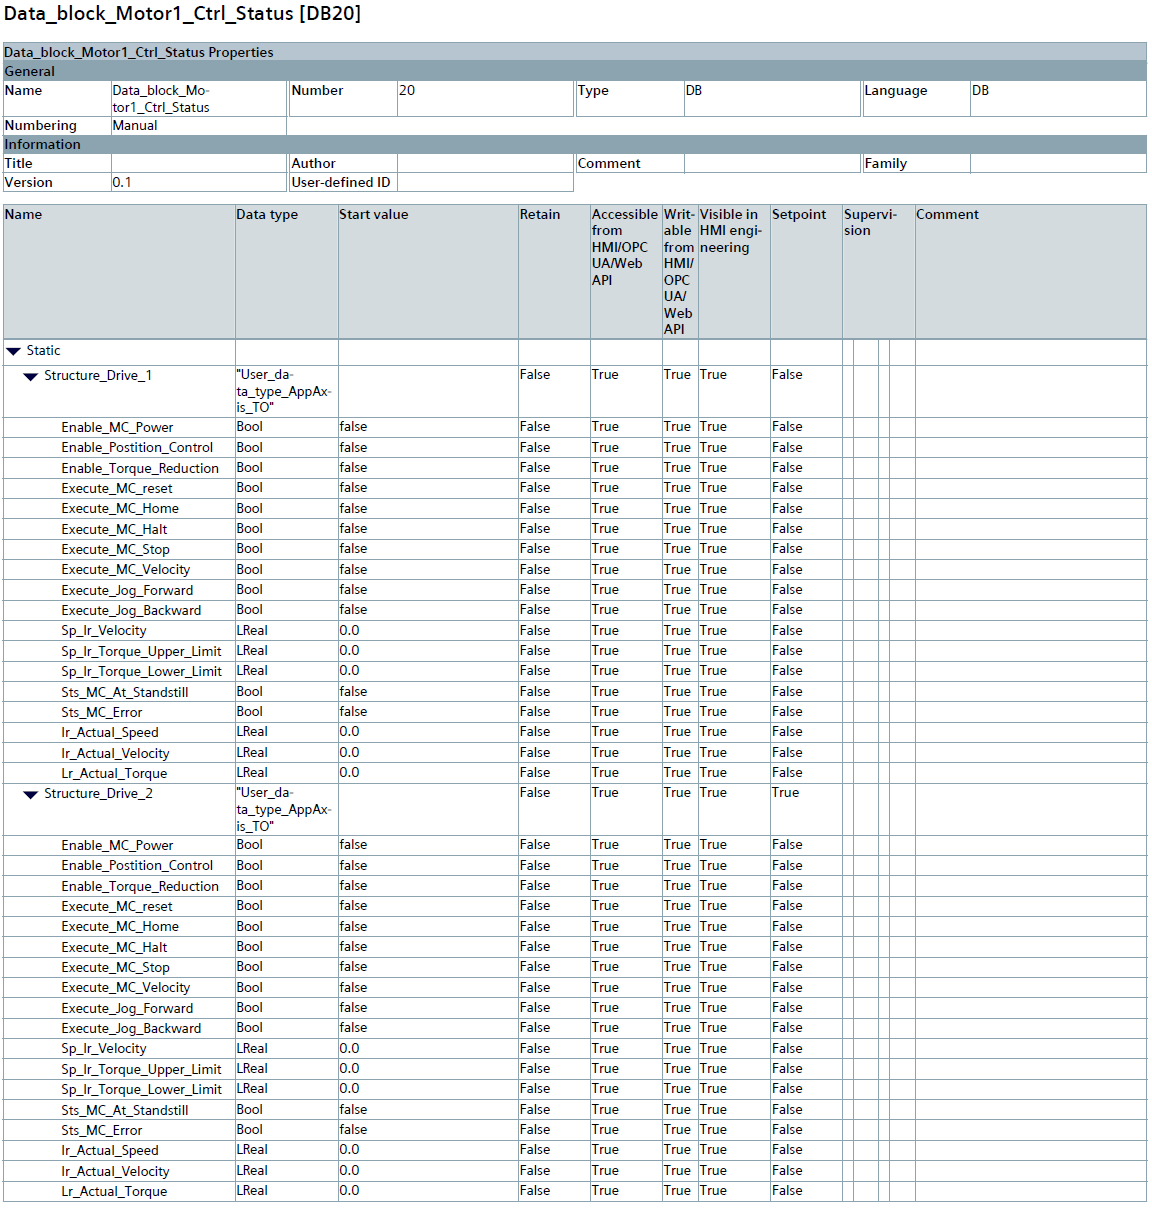
\includegraphics[width=0.5\linewidth]{DBs/MotorCtrlStatus.PNG}
    \caption{Datablokk for å holde statusverdiene til begge motordrivene på \acrshort{pls}-en.}
    \label{fig:MotorSTS}
\end{figure}
\begin{figure}[H]
    \centering
    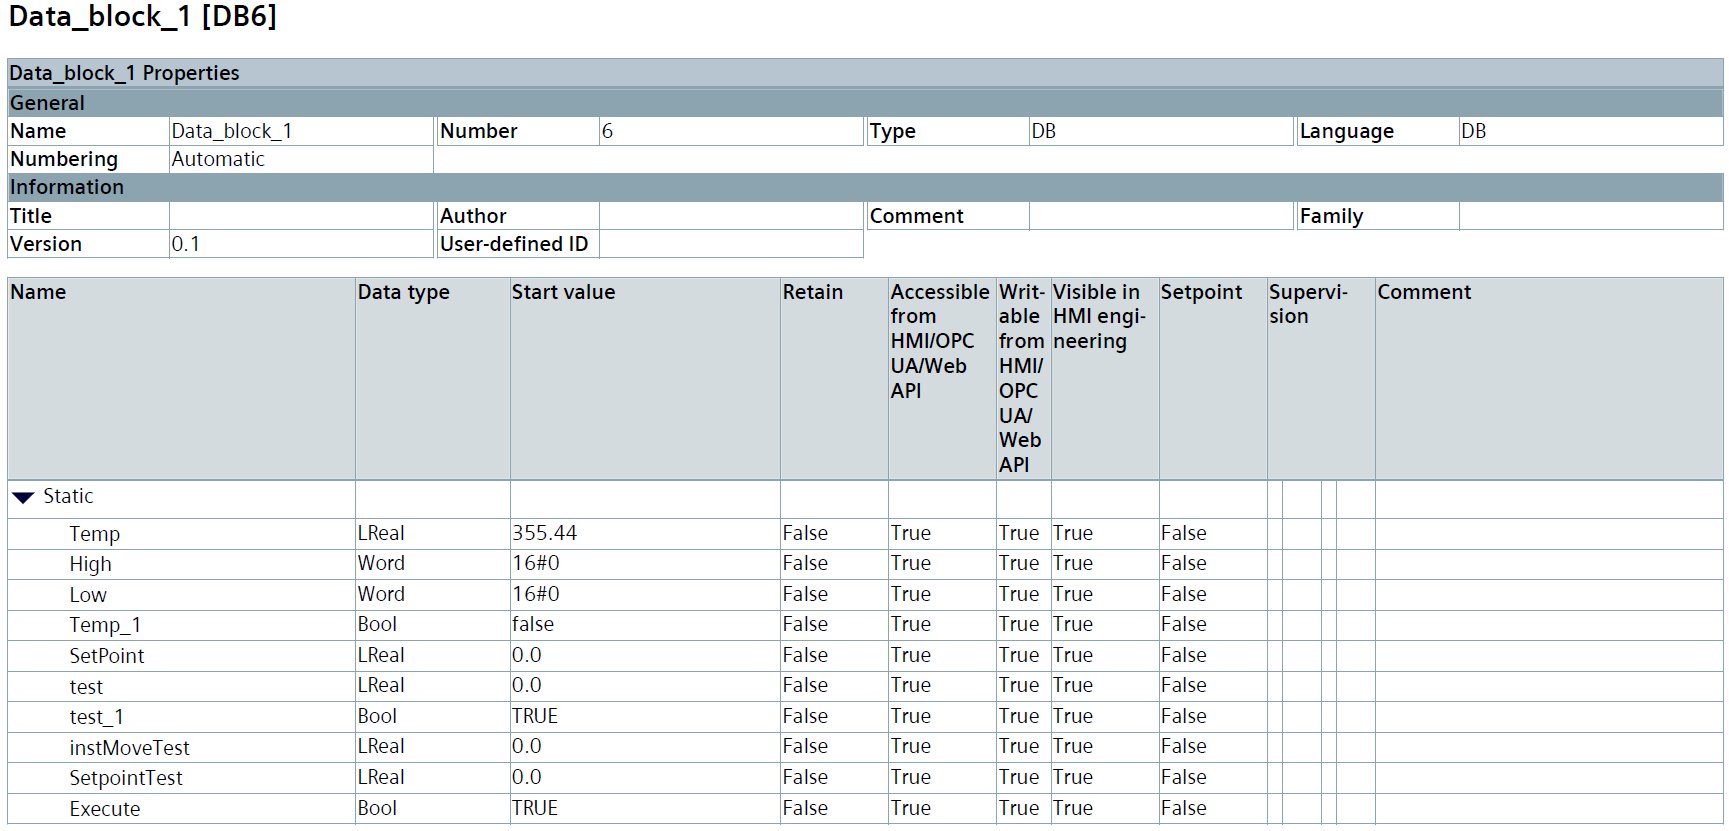
\includegraphics[width=0.5\linewidth]{DBs/temp.PNG}
    \caption{Datablokk som holder midlertidige verdier for \acrshort{pls}-aritmetikk og testverdier.}
    \label{fig:temp}
\end{figure}
\clearpage
\section{Labview}

\subsection{Typedefs}
\begin{multicols}{2}
\begin{figure}[H]
    \centering
    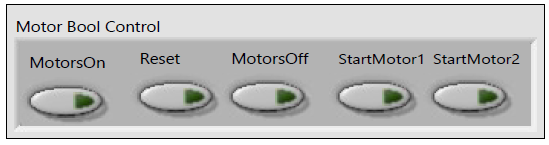
\includegraphics[width=0.5\linewidth]{vis/Motor Bool control.PNG}
    \caption{\Gls{type} av de \glspl{boolean} sendt over Modbus-tilkoblingen.}
    \label{fig:MotorBoolCl}
\end{figure}
\begin{figure}[H]
    \centering
    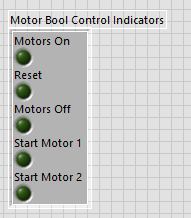
\includegraphics[width=0.5\linewidth]{vis/Motor Bool Indicatorsl.PNG}
    \caption{\Gls{type} av de \glspl{boolean} mottatt over Modbus-tilkoblingen.}
    \label{fig:MotorBoolInd}
\end{figure}
\begin{figure}[H]
    \centering
    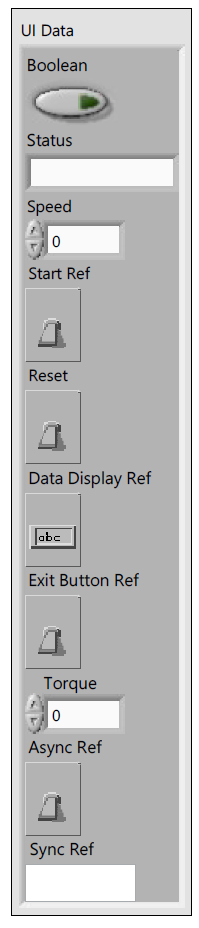
\includegraphics[scale=0.5]{vis/UI.PNG}
    \caption{\Gls{type} av elementene i \glset{bg}.}
    \label{fig:UI}
\end{figure}
\end{multicols}
\subsection{Helper VIs}
\begin{figure}[H]
    \centering
    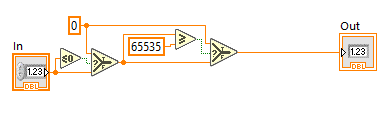
\includegraphics[width=0.5\linewidth]{vis/Remove invalid values.PNG}
    \caption{\textit{RemoveInvalidValues.vi} er en hjelpe \Gls{vi} som fjerner ugyldige verdier. Fordi en 16-bit \gls{word}, uten fortegn som blir send over Modbus-tilkoblingen kun kan ha heltallsverdier mellom $0$ og $2^{16} = 65535$. Any value outside this range is forced to be either $0$ or $65535$.}
    \label{fig:RIV}
\end{figure}
\begin{figure}[H]
    \centering
    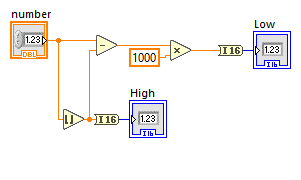
\includegraphics[width=0.5\linewidth]{vis/SplitDouble.PNG}
    \caption{\textit{SplitDouble.vi} is a helper VI that splits a 64 bit-double into two 16-bit words \textbf{High} and \textbf{Low} for Modbus communication. The double is first rounded down to a integer to get the \textbf{High}-part and then that is subtracted from the original number the remaining \textbf{Low}-part is then multiplied by $1000$ because you can't send decimals on this form. On the receiving side the \textbf{Low}-part is divided by $1000$ again as shown in \figref{fig:Splice}.}
    \label{fig:SplitDouble}
\end{figure}

\begin{figure}[H]
    \centering
    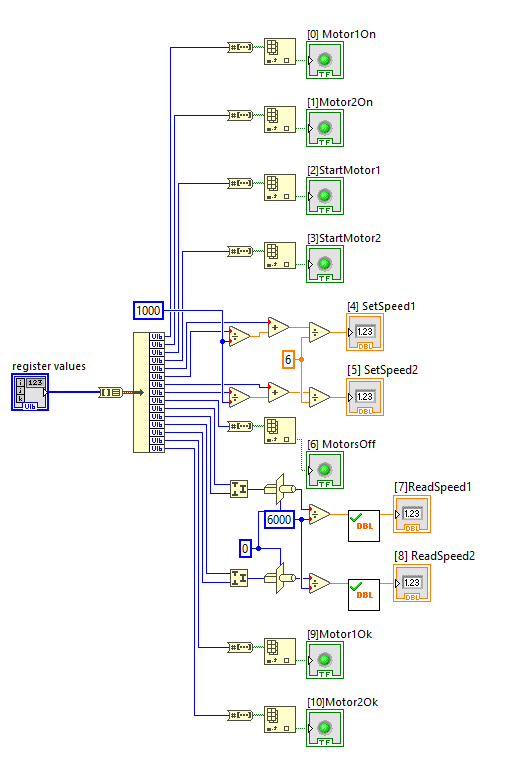
\includegraphics[width=0.5\linewidth]{vis/RegisterSplit.PNG}
    \caption{\textit{RegisterSplit.vi} is a helper VI that splits the register received over modbus to appropriate values for the Labview application.}
    \label{fig:RegisterSplit}
\end{figure}

\subsection{Important VIs}
\begin{figure}[H]
    \centering
    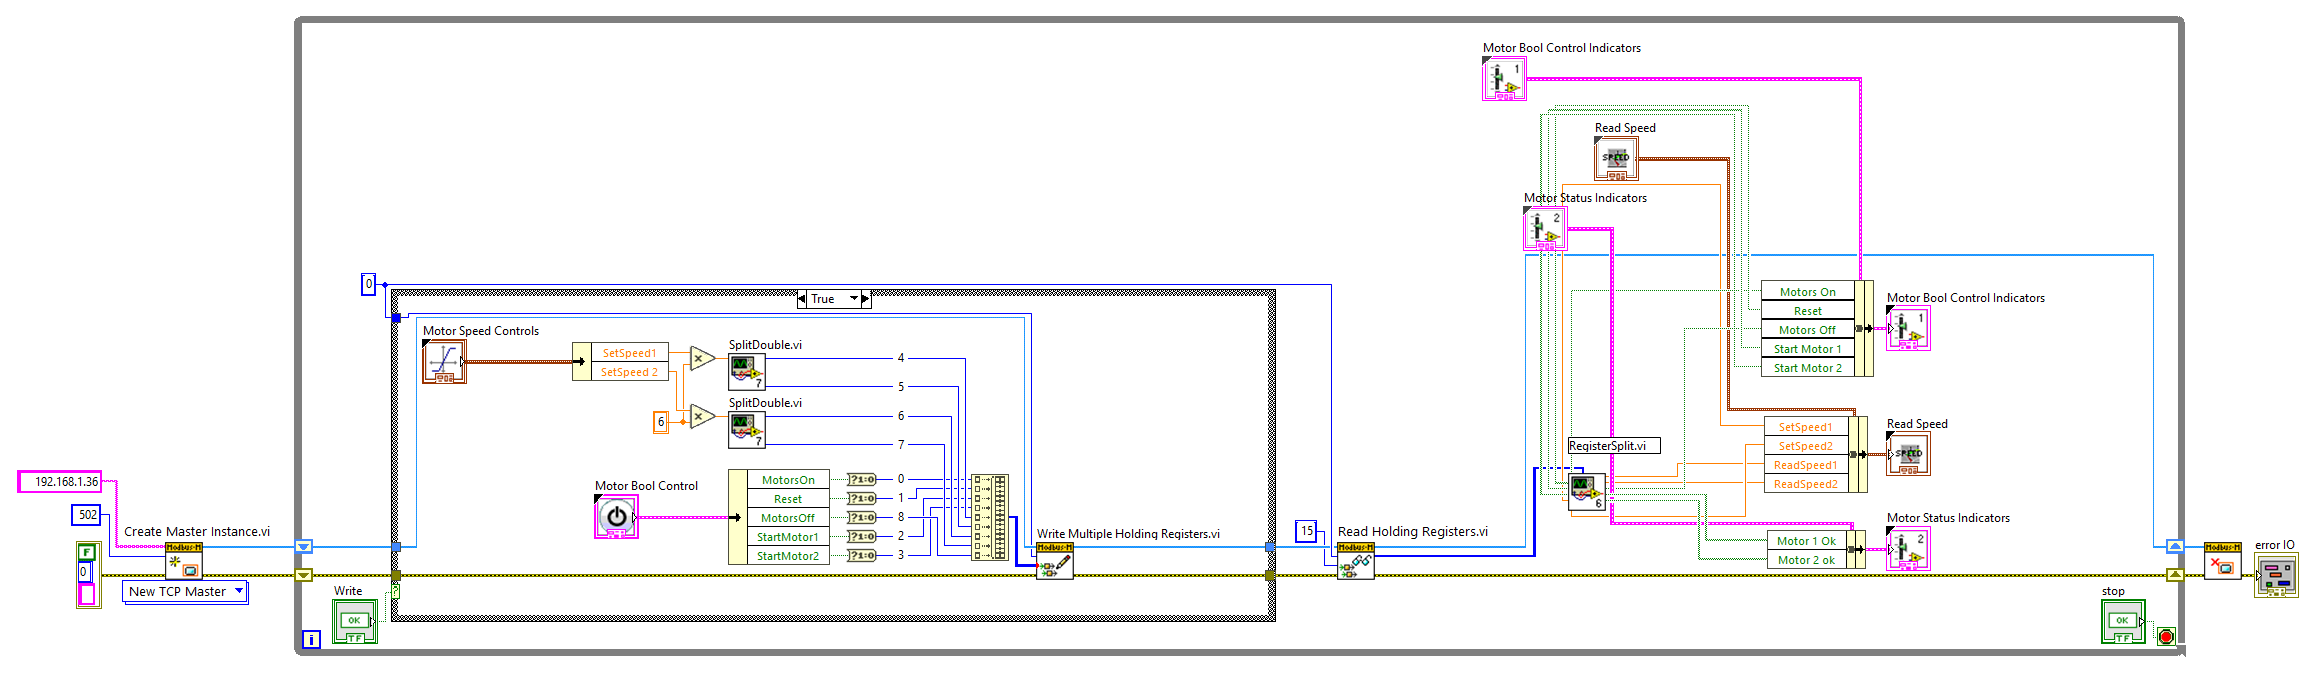
\includegraphics[width=0.75\linewidth]{vis/ModbusIO.PNG}
    \caption{How the modbus connection works on the labview side. This has been adapted to fit better into the \acrshort{mcl}, but functionality is the same.}
    \label{fig:ModbusIO}
\end{figure}

\begin{figure}[H]
    \centering
    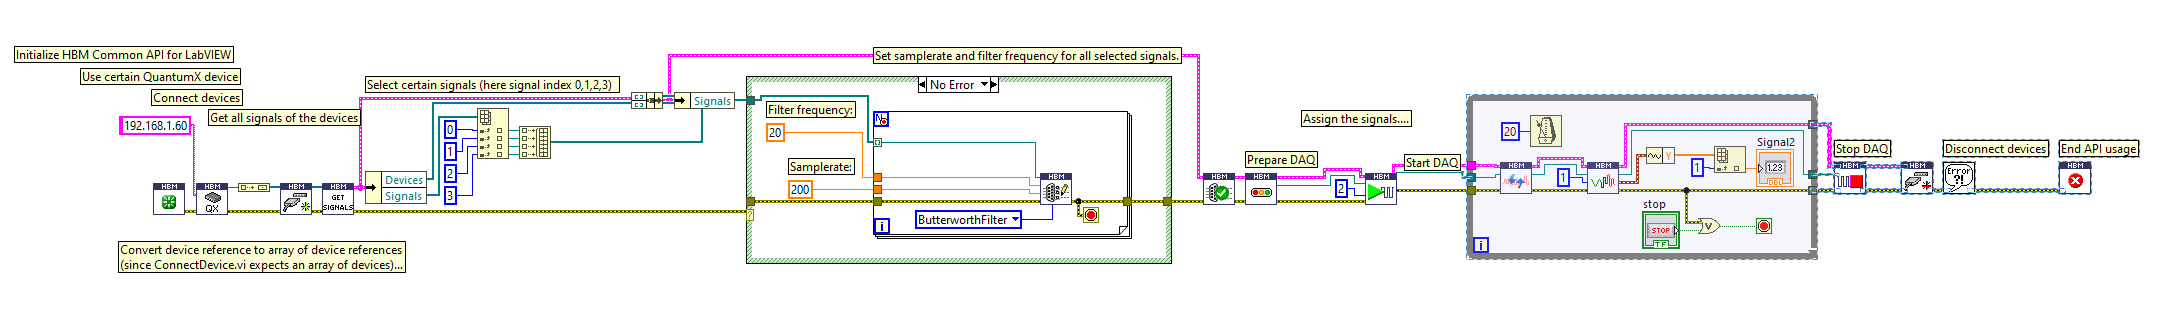
\includegraphics[width=0.75\linewidth]{vis/LoggingSystem.PNG}
    \caption{How the loggin system works. This has been adapted to fit better into the logging loop, but functionality is the same. This example also takes measurements from one channel, the full system utilises all four available channels.}
    \label{fig:Logging}
\end{figure}
\end{document}
